\newpage
\section{Auswertung}
\subsection{Erdmagnetfeld und Landé-Faktoren}
\label{sec:Auswertung}
% \subsection{Unterkapiel}
% \label{sec:Unterkapitel}

% \begin{figure}
%   \centering
%   \includegraphics[width=\textwidth]{Plot.pdf}
%   \caption{Bildunterschrift}
%   \label{fig:Plot1}
% \end{figure}
\FloatBarrier
Die Magnetfelder werden aus der Formel
\begin{equation}
B=\mu_0\frac{8 I N}{\sqrt{125}R}
\end{equation}
für Helmholtzspulen errechnet.
Hierbei ist $I$ die abgelesene Stromstärke, $N$ die Anzahl der Windungen und $R$ der Radius der Spule.

Zunächst wird die vertikale Komponente $B_{\text{vert}}$ des Erdmagnetfeldes kompensiert.
Das dafür angelegte Magnetfeld beträgt
\begin{equation}
B_{\text{vert}}=\SI{3.448e-5}{\tesla}
\end{equation}
wofür der aufgenommene Peak minimal wird.
Ein typisches Signalbild ist in Abbildung \ref{fig:Signal} zu sehen.
 \begin{figure}
   \centering
   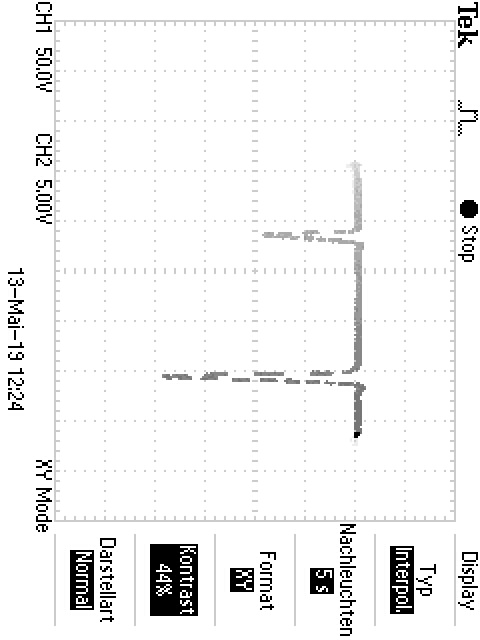
\includegraphics[width=10cm]{pictures/TEK0008.JPG}
   \caption{Typisches Signal am Oszilloskop.}
   \label{fig:Signal}
 \end{figure}
 \FloatBarrier

Die Resonanzpositionen sind in Tabelle \ref{tab:RF} einzusehen und in Abbildung zusätzlich zu einem linearen Fit graphisch dargestellt.
Die lineare Regression hat die Form
\begin{equation*}
B=a\nu_{\text{RF}}+b.
\end{equation*}
Ein Blick auf Formel \ref{eqn:B} verrät, dass 
\begin{equation*}
a=\frac{h}{\mu_{\text{B}}g_{\text{F}}}
\end{equation*}
und damit 
\begin{equation*}
g_{\text{F}}=\frac{h}{\mu_{\text{B}}a}
\end{equation*}
gilt.
Aus der ersten Resonanzstelle ergibt sich
\begin{align*}
a&=(142.1\pm0.9)\num{e-6}\frac{\si{\tesla}}{\si{\mega\hertz}}\\
b&=(19.9\pm0.5)\num{e-6}\si{\tesla}\\
\Rightarrow g_{\text{F,1}}&=0.502\pm0.003
\end{align*}
und aus der zweiten
\begin{align*}
a&=(212\pm1)\num{e-6}\frac{\si{\tesla}}{\si{\mega\hertz}}\\
b&=(20.2\pm0.6)\num{e-6}\si{\tesla}\\
\Rightarrow g_{\text{F,2}}&=0.336\pm0.001.
\end{align*}
Somit ergibt sich das Verhältnis der beiden Faktoren zu
\begin{equation*}
\frac{g_{\text{F,1}}}{g_{\text{F,2}}}=1.49\pm0.01.
\end{equation*}
Die horizontale Komponente des Erdmagnetfeldes lässt sich aus dem Fitparameter $b$ auslesen.
Der Mittelwert der berechneten Werte beträgt
\begin{equation*}
 B_{\text{hor}}=(2.01\pm0.04)e-5\si{\tesla}.
\end{equation*}
\begin{table}[h]
  \centering
  \begin{tabular}{S[table-format=1.1] S S}
    {$\nu_\text{RF}$ / MHz} & {$B_1$ / µT} & {$B_2$ / µT} \\
    \midrule
    0.1 &  33.98&   41.28 \\
    0.2 &  48.93 &   63.35 \\
    0.3 &  62.62 &   83.99 \\
    0.4 &  76.17 &  104.59 \\
    0.5 &  90.02 &  125.44 \\
    0.6 & 105.82 &  149.33 \\
    0.7 & 120.44 &  170.10 \\
    0.8 & 134.89 &  190.48 \\
    0.9 & 147.53 &  210.25 \\
    1.0 & 161.26 &  233.12
  \end{tabular}
  \caption{Resonanzpositionen abhängig von der RF-Frequenz.}
  \label{tab:RF}
\end{table}
 \begin{figure}
   \centering
   \includegraphics[width=\textwidth]{build/B.pdf}
   \caption{Frequenz gegen B-Feldstärke der Resonanzstellen aufgetragen.}
   \label{fig:B.pdf}
 \end{figure}
 \FloatBarrier
 \subsection{Kernspins}
 Die Quantenzahlen für Rubidium betragen
 \begin{equation*}
 L = 0,\quad S = \frac{1}{2},\quad J = \frac{1}{2}
 \end{equation*}
 wodurch mit Hilfe von Gleichung \ref{eqn:gj} sich der Faktor
 \begin{equation*}
 g_{\text{J}}=2.0023
 \end{equation*}
 ergibt.
 Einsetzen von $F=I+J$ in \ref{eqn:lande} und umformen nach dem Kernspin $I$ ergibt
 \begin{equation}
 I=\frac{g_J-4g_F}{4g_F} + \sqrt{\left(\frac{g_J-4g_F}{4g_F}\right)^2-\frac{3}{4}\left(1-\frac{g_J}{g_F}\right)}.
 \end{equation}
 Mit den vorher berechneten Werten der Landéschen Faktoren ergibt sich
 \begin{align*}
 I_1 &= 1.49 \pm 0.01\\
 I_2 &= 2.57 \pm 0.01 
 \end{align*}
 für die Kernspins.
 Der Vergleich mit der Literatur \cite{nudat2}
\begin{align*}
{}^{87}\text{Rb}:\quad I&=\frac{3}{2}\\
\\
{}^{85}\text{Rb}:\quad I&=\frac{5}{2}
\end{align*}
verrät, dass die erste Resonanz zum Isotop $\ce{^{87}Rb}}$ gehört und die zweite zum Isotop $\ce{^{85}Rb}}$.
\subsection{Isotopenverhältnis}
Aus Abbildung \ref{fig:Signal} wird das Verhältnis der Amplituden zueinander ausgemessen.
Da die genaue Messung mit dem Oszilloskop nicht erfolgt ist, wird versucht die Amplitudentiefe per Gimp zu erfassen.
Die Höhen der Amplituden entsprechen
\begin{align*}
h_1&=(92.0\pm0.9)\text{px}\\
h_2&=(192\pm2)\text{px}
\end{align*}
mit einem Messfehler von \SI{1}{\percent}.
Damit ergibt sich ein Verhältnis von
\begin{equation}
  \frac{h_1}{h_2}=0.479\pm0.006.
\end{equation}
Aus der Literatur \cite{nudat2} wird das Verhältnis zu 
\begin{equation}
  \frac{h_1}{h_2}=0.39
\end{equation}
bestimmt.
\subsection{Quadratischer Zeeman-Effekt}
Die Effekte des quadratischen Zeemaneffekts werden aus Gleichung \ref{eqn:zeemanquadrat} hergeleitet.
Die für die Rechnung benutzten Werte sind in Tabelle \ref{tab:qZ} angegeben.
\begin{align*}
{}^{87}\text{Rb}: U_{\text{Z}}&=(7.52\pm0.05)\num{e-28}\si{\joule}\\
{}^{85}\text{Rb}: U_{\text{Z}}&=(7.27\pm0.04)\num{e-28}\si{\joule}
\end{align*}
\begin{table}
  \centering
  \caption{Werte zur Bestimmung des quadratischen Zeemaneffekts.}
  \label{tab:qZ}
  \begin{tabular}{c c S[table-format=1.2e2] S[table-format=1.4] @{${}\pm{}$} S[table-format=1.4] S[table-format=3.0]}
    Isotop & $M_F$ & {$\symup{\Delta}E_\text{Hy}$ / J} & \multicolumn{2}{c}{$g_F$} & {$B$ / µT} \\
    \midrule
    ${}^{85}$Rb & 0 & 2.01e-24 & 0.3361 & 0.0017 & 233.12 \\
    ${}^{87}$Rb & 0 & 4.53e-24 & 0.5026 & 0.0032 & 161.26 \\
  \end{tabular}
\end{table}